\chapter{الأمواج على الأوتار والقضبان: معادلة دالمبير}\label{ch:b2:waves-on-strings}

اقطف وتر قيثارة فيجري شكل على امتداده، ويرتدّ عن الفرس،
ويعود، ويستقر في النقش المستقر الذي تسمع تواتره نغمةً. وضع
أذنك على قضيب سكة حديدية فتسمع القطار قبل وصوله بكثير: إذ
يجري انضغاط في الفولاذ بخمسة كيلومترات في الثانية. وقد وصف
كتاب السنة الأولى مثل هذه الأمواج --- منتقلةً ومستقرةً
ومتراكبةً --- دون أن يقول لماذا توجد. وهذا الفصل يشتقّ
المعادلة التي تحكمها، أي \emph{\omterm{thm:b2:waves-on-strings:equation}{معادلة دالمبير} للأمواج}، من أجل
الحركة المستعرضة لوتر أولًا، ثم من أجل الحركة الطولية لقضيب
مبنيّ، ذرّةً ذرّةً، من كتل ونوابض؛ ويحسب الطاقة التي تحملها
الموجة والممانعة التي تقرّر ما يحدث حين تلقى تغيّرًا في الوسط.

\section{الوتر المهتزّ}

\begin{theorem}[معادلة الأمواج في وتر]\label{thm:b2:waves-on-strings:equation}
\index{معادلة دالمبير}\index{معادلة الأمواج}\index{سرعة الموجة (وتر)}
وتر كثافته الطولية $\mu$، مشدود بتوتر $T$، يقوم بانتقالات
مستعرضة صغيرة $y(x, t)$ (وميوله $|\partial_xy| \ll 1$). عندئذ
\[
\frac{\partial^2y}{\partial t^2} = c^2\,\frac{\partial^2y}{\partial x^2} ,
\qquad c = \sqrt{\frac{T}{\mu}} ,
\]
وهي \emph{\omterm{thm:b2:waves-on-strings:equation}{معادلة دالمبير}}، وحلّها العام $y = f(x - ct)
+ g(x + ct)$: أي تراكب شكل ينتقل نحو اليمين وشكل ينتقل نحو
اليسار بالسرعة $c$، دون تشوّه.
\end{theorem}

\begin{proof}
لنعزل العنصر بين $x$ و $x + \dd x$، وكتلته $\mu\,\dd x$. فيجذبه
جاراه على امتداد مماس الوتر بالتوتر $T$:
أفقيًّا $T\cos\theta \approx T$ عند الطرفين (إذ لا حركة أفقية، ومنه
يكون $T$ واحدًا على امتداده)، وشاقوليًّا $T\sin\theta \approx T\partial_xy$، وهو ما
يعطي القوة الصافية $T[\partial_xy(x + \dd x) - \partial_xy(x)] = T\,\partial_x^2y\,\dd x$.
ونيوتن: $\mu\,\dd x\,\partial_t^2y = T\partial_x^2y\,\dd x$. وأما الحلّ، فنضع
$u = x - ct$ و $v = x + ct$: فتصير المعادلة $\partial_u\partial_vy = 0$
(بقاعدة الاشتقاق المركّب)، ومنه لا يتوقف $\partial_vy$ إلا على $v$، ويكون $y = f(u) + g(v)$؛
وبالعكس يحققها كل $y$ من هذا الشكل. وأما الثقالة، وقد أُهملت، فذلك مشروع
حين $T \gg \mu gL$.
\end{proof}

\begin{omfigure}
\begin{tikzpicture}[font=\small, x=1cm, y=1cm, >=Stealth]
  \begin{scope}
    \draw[->] (-2.5,0) -- (3.0,0) node[right, font=\footnotesize] {$x$};
    \draw[omDef, very thick, domain=-2.3:2.8, samples=60] plot (\x,{0.9*exp(-(\x)^2/1.6)});
    \coordinate (A) at (-0.6,{0.9*exp(-0.36/1.6)}); \coordinate (B) at (0.2,{0.9*exp(-0.04/1.6)});
    \fill[omThm] (A) circle (1.5pt); \fill[omThm] (B) circle (1.5pt);
    \draw[omThm, very thick, ->] (A) -- ($(A)+(-0.9,-0.55)$) node[above left, font=\footnotesize, yshift=2pt] {$\vect T(x)$};
    \draw[omThm, very thick, ->] (B) -- ($(B)+(1.0,-0.12)$) node[right, font=\footnotesize] {$\vect T(x+\dd x)$};
    \draw[dashed] (-0.6,0) -- (A); \draw[dashed] (0.2,0) -- (B);
    \node[font=\footnotesize] at (-0.6,-0.3) {$x$}; \node[font=\footnotesize] at (0.35,-0.3) {$x + \dd x$};
    \node[font=\footnotesize] at (0.2,-0.9) {$\mu\,\dd x\,\partial_t^2y = T\,\partial_x^2y\,\dd x$};
  \end{scope}
  \begin{scope}[xshift=7.6cm]
    \draw[->] (-2.5,0) -- (3.0,0) node[right, font=\footnotesize] {$x$};
    \draw[omDef, thick, domain=-2.3:2.8, samples=60] plot (\x,{0.8*exp(-(\x+1.3)^2/0.5)});
    \draw[omDef, thick, dashed, domain=-2.3:2.8, samples=60] plot (\x,{0.8*exp(-(\x-0.5)^2/0.5)});
    \draw[omDef, thick, ->] (-1.0,1.0) -- (0.2,1.0) node[above, font=\footnotesize, pos=0.5] {$c$};
    \node[font=\footnotesize] at (-1.3,-0.35) {$t$}; \node[font=\footnotesize] at (0.5,-0.35) {$t + \tau$};
    \node[font=\footnotesize] at (0.2,-0.9) {$y = f(x - ct)$};
  \end{scope}
\end{tikzpicture}

{\small على اليسار: القوى على عنصر من الوتر --- فالتوتران
ليسا متوازيين حين يكون الوتر منحنيًا، ومحصّلتهما
مستعرضة. وعلى اليمين: شكل $f(x - ct)$ ينتقل نحو اليمين بالسرعة $c$
دون تشوّه.}
\end{omfigure}

\begin{example}[القيثارة والبيانو والكابل]\label{ex:b2:waves-on-strings:numbers}
وتر مي الغليظ في قيثارة ($\mu = \qty{5.5}{g/m}$، وطوله \qty{0.65}{m}،
و \qty{82.4}{Hz}) يهتزّ في نمطه الأساسي بطول موجة $\lambda = 2L$: فيكون $c = 2Lf =
\qty{107}{m/s}$ و $T = \mu c^2 = \qty{63}{N}$. ووتر لا$_4$ في بيانو (فولاذ،
\qty{1}{mm}، و $\mu = \qty{6.1}{g/m}$، و \qty{0.38}{m}، و \qty{440}{Hz}): $c = \qty{334}{m/s}$،
و $T = \qty{680}{N}$ --- وفي البيانو نحو $230$ وترًا، أي عشرون
طنًّا من التوتر على إطار من الحديد الصبّ. وكابل كثافته \qty{1}{kg/m} عند \qty{10}{kN}:
\qty{100}{m/s}.
\end{example}

\section{الأمواج المستقرة والأنماط}

\begin{proposition}[أنماط وتر مثبَّت من طرفيه]\label{prop:b2:waves-on-strings:modes}
\index{أنماط ذاتية}\index{توافقيات}\index{موجة مستقرة}
وتر مثبَّت عند $x = 0$ و $x = L$ يقبل حلول الأمواج المستقرة
الجيبية (أي \emph{\omterm{prop:b2:waves-on-strings:modes}{الأنماط الذاتية}})
\[
y_n(x, t) = A_n\sin\frac{n\pi x}{L}\cos(\omega_nt - \varphi_n) , \qquad
f_n = \frac{\omega_n}{2\pi} = n\,\frac{c}{2L} = n f_1 , \quad n = 1, 2, 3, \dots
\]
--- أي النمط الأساسي $f_1 = c/2L$ و\emph{توافقياته}. وللنمط $n$
عدد $n - 1$ من العقد بين الطرفين. وكل حركة للوتر تراكب
$y = \sum_ny_n$، والسعات والأطوار تحدّدها الحالة الابتدائية
شكلًا وسرعةً (وهي متسلسلة فورييه، كما يقرّر كتاب الرياضيات
لهذه السنة): ومزيج التوافقيات هو \emph{جرس} النغمة.
\end{proposition}

\begin{proof}
لنبحث عن $y = F(x)\cos(\omega t - \varphi)$: فيكون $F'' + (\omega/c)^2F = 0$، ويعطي $F(0) = 0$
الحلّ $F = A\sin(\omega x/c)$، ويقتضي $F(L) = 0$ أن يكون $\omega L/c = n\pi$. وكل نمط
مجموع موجتين منتقلتين كذلك: $\sin kx\cos\omega t = \tfrac12[\sin(kx -
\omega t) + \sin(kx + \omega t)]$ --- أي الموجة وانعكاسها. وأما
تمام جملة الجيوب فمبرهنة فورييه.
\end{proof}

\begin{omfigure}
\begin{tikzpicture}
\begin{axis}[omaxis, axis x line=bottom, axis y line=none, width=6.4cm, height=5.2cm,
    xmin=0, xmax=1, ymin=-5.9, ymax=1.5, xtick={0,1}, xticklabels={$0$, $L$}, samples=80,
    xlabel={}, ylabel={}]
  \addplot[omDef, thick, domain=0:1] {sin(deg(pi*x))};
  \addplot[omDef, thick, dashed, domain=0:1] {-sin(deg(pi*x))};
  \addplot[omThm, thick, domain=0:1] {0.8*sin(deg(2*pi*x))-2.6};
  \addplot[omThm, thick, dashed, domain=0:1] {-0.8*sin(deg(2*pi*x))-2.6};
  \addplot[omProp, thick, domain=0:1] {0.7*sin(deg(3*pi*x))-5.0};
  \addplot[omProp, thick, dashed, domain=0:1] {-0.7*sin(deg(3*pi*x))-5.0};
  \addplot[black, thin] coordinates {(0,-2.6) (1,-2.6)};
  \addplot[black, thin] coordinates {(0,-5.0) (1,-5.0)};
  \node[font=\scriptsize] at (axis cs:0.5,1.25) {$n = 1$};
  \node[font=\scriptsize] at (axis cs:0.5,-1.4) {$n = 2$};
  \node[font=\scriptsize] at (axis cs:0.5,-3.85) {$n = 3$};
\end{axis}
\end{tikzpicture}
\hfill
\begin{tikzpicture}
\begin{axis}[omaxis, axis x line=bottom, axis y line=left, width=5.0cm, height=4.2cm,
    xlabel={$x/L$}, ylabel={$y$}, xmin=0, xmax=1, ymin=-0.05, ymax=1.1, xtick={0,0.5,1}, ytick=\empty, samples=200, clip=false,
    xlabel style={at={(axis description cs:0.5,-0.12)}, anchor=north},
    ylabel style={at={(axis description cs:-0.06,0.5)}, rotate=90, anchor=south}]
  \addplot[black, thick] coordinates {(0,0) (0.5,1) (1,0)};
  \addplot[omDef, thick, domain=0:1] {0.81*sin(deg(pi*x))};
  \addplot[omThm, thick, domain=0:1] {0.81*sin(deg(pi*x)) - 0.09*sin(deg(3*pi*x))};
  \node[font=\scriptsize, anchor=west] at (axis cs:0.03,0.95) {مقطوف};
  \node[font=\scriptsize, omDef, anchor=east] at (axis cs:0.97,0.95) {$n = 1$};
  \node[font=\scriptsize, omThm, anchor=east] at (axis cs:0.97,0.78) {$n = 1, 3$};
\end{axis}
\end{tikzpicture}

{\small على اليمين: الأنماط الثلاثة الأولى لوتر مثبَّت من طرفيه ($f_n = nc/2L$).
وعلى اليسار: وتر مقطوف في منتصفه (مثلث) والحدود الأولى
من متسلسلة فورييه له --- فلا تظهر إلا التوافقيات الفردية، وسعاتها
تهبط مثل $1/n^2$.}
\end{omfigure}

\begin{example}[تجربة ملد]\label{ex:b2:waves-on-strings:melde}
\index{تجربة ملد}
وتر يُهزّ من أحد طرفيه بهزّاز عند التواتر $f$، وطرفه الآخر
يمرّ فوق بكرة إلى كتلة معلَّقة $m$ (ومنه $T = mg$): فتظهر \omterm{prop:b2:waves-on-strings:modes}{موجة
مستقرة} كبيرة كلما ساوى $f$ أحد $f_n = (n/2L)
\sqrt{mg/\mu}$ --- أي رنين النمط $n$. ومن أجل $L = \qty{1.2}{m}$، و $\mu =
\qty{1.0}{g/m}$، و $f = \qty{50}{Hz}$، تكون الكتل التي تعطي $n = 1, 2, 3$ عروة
هي $m_n = 4L^2f^2\mu/n^2g = 1.47/n^2$ كيلوغرام: أي \qty{1.47}{kg}، و \qty{367}{g}، و \qty{163}{g}.
والضغط على وتر قيثارة عند الدستان الثاني عشر ينصّف $L$ ويضاعف
$f_1$: أي الديوان؛ ولمسه لمسًا خفيفًا في المنتصف دون ضغط
يقتل الأنماط الفردية ويترك التوافقي الثاني --- وهي النغمة التوافقية.
\end{example}

\section{الطاقة والاستطاعة والممانعة}

\begin{proposition}[طاقة موجة على وتر]\label{prop:b2:waves-on-strings:energy}
\index{كثافة الطاقة (وتر)}\index{تدفق الطاقة (وتر)}\index{ممانعة (وتر)}
يحمل الوتر الطاقة في واحدة الطول والاستطاعة (أي تدفق الطاقة
نحو $+x$)
\[
e = \tfrac12\mu\Bigl(\frac{\partial y}{\partial t}\Bigr)^2 + \tfrac12T\Bigl(\frac{\partial y}{\partial x}\Bigr)^2 ,
\qquad
\mathcal P = -T\,\frac{\partial y}{\partial x}\,\frac{\partial y}{\partial t} ,
\]
وهما تحققان الموازنة الموضعية $\partial_te + \partial_x\mathcal P = 0$. ومن أجل
موجة متقدمة $y = f(x - ct)$، تتساوى الكثافتان الحركية والكامنة
ويكون $\mathcal P = Z\,(\partial_ty)^2$ حيث
\[
Z = \sqrt{T\mu} = \mu c = \frac Tc ,
\]
وهي \emph{ممانعة} الوتر (\unit{kg/s}): أي نسبة القوة
المستعرضة $-T\partial_xy$ التي يؤثر بها الوتر فيما هو أمامه
إلى السرعة المستعرضة $\partial_ty$. وموجة جيبية سعتها $A$
تحمل الاستطاعة الوسطى $\langle\mathcal P\rangle = \tfrac12Z\omega^2A^2$.
\end{proposition}

\begin{proof}
الحدّ الكامن هو شغل التوتر وهو يمطّ العنصر:
إذ طوله
\[
\dd x\sqrt{1 + (\partial_xy)^2} \approx \dd x\bigl(1 + \tfrac12(\partial_xy)^2\bigr) ,
\]
ومنه يعطي فائض الطول مضروبًا في $T$ المقدارَ $\tfrac12T(\partial_xy)^2\dd x$. والاستطاعة
المنقولة عبر $x$ نحو $+x$ هي القوة المستعرضة التي يؤثر بها
الجزء الأيسر في الجزء الأيمن، $-T\partial_xy$، مضروبةً في السرعة
$\partial_ty$. والموازنة:
\[
\partial_te = \mu\,\partial_ty\,\partial_t^2y + T\,\partial_xy\,\partial_x\partial_ty ,
\qquad
-\partial_x\mathcal P = T\,\partial_x^2y\,\partial_ty + T\,\partial_xy\,\partial_x\partial_ty ,
\]
وهما متساويان \omterm{thm:b2:waves-on-strings:equation}{بمعادلة الأمواج}. ومن أجل $f(x - ct)$: $\partial_xy = -\partial_ty/c$، ومنه $\mathcal P = (T/c)
(\partial_ty)^2$ وتساوي الكثافتان $\tfrac12\mu(\partial_ty)^2$.
\end{proof}

\begin{proposition}[الانعكاس والنفاذ عند وصلة]\label{prop:b2:waves-on-strings:junction}
\index{معامل الانعكاس (وتر)}\index{معامل النفاذ (وتر)}
موجة سعتها $A_i$ تصل من وتر ممانعته $Z_1$ إلى
وتر ممانعته $Z_2$ موصولين عند $x = 0$. ويعطي اتصال
الانتقال والقوة المستعرضة عند الوصلة معاملي
السعة
\[
r = \frac{A_r}{A_i} = \frac{Z_1 - Z_2}{Z_1 + Z_2} , \qquad
t = \frac{A_t}{A_i} = \frac{2Z_1}{Z_1 + Z_2} ,
\]
والنسبتين الطاقيتين $R = r^2$ و $\mathcal T = 4Z_1Z_2/(Z_1 + Z_2)^2$، مع
$R + \mathcal T = 1$. والطرف المثبَّت ($Z_2 \to \infty$) يعكس بالمعامل $r = -1$
(فتعود النبضة مقلوبة)، والطرف الحرّ ($Z_2 = 0$) بالمعامل $r = +1$؛
والممانعتان المتساويتان تنفذان كل شيء.
\end{proposition}

\begin{proof}
موجتان جيبيتان $y_1 = A_i\cos(\omega t - k_1x) + A_r\cos(\omega t + k_1x)$ من أجل
$x < 0$، و $y_2 = A_t\cos(\omega t - k_2x)$ من أجل $x > 0$، و $\omega$ نفسها على
الجانبين. وعند $x = 0$: يعطي $y_1 = y_2$ العلاقة $A_i + A_r = A_t$؛ ويعطي اتصال القوة $-T\partial_xy$
(والوصلة معدومة الكتلة) العلاقة $Z_1(A_i - A_r) = Z_2A_t$ (باستعمال
$T_1k_1 = Z_1\omega$). ثم نحلّ. وأما الطاقات: فبالاستطاعات الوسطى $\tfrac12Z\omega^2A^2$.
\end{proof}

\begin{omfigure}
\begin{tikzpicture}[font=\small, x=1cm, y=1cm, >=Stealth]
  \begin{scope}
    \draw[->] (-3.2,0) -- (3.2,0) node[right, font=\footnotesize] {$x$};
    \draw[omDef, very thick, domain=-3.0:0, samples=50] plot (\x,{0.8*exp(-(\x+1.6)^2/0.25)});
    \draw[omDef, very thick, domain=0:3.0, samples=50] plot (\x,{0});
    \fill (0,0) circle (2pt); \node[font=\footnotesize] at (0,-0.35) {$Z_1 \to Z_2$};
    \draw[omDef, ->, thick] (-1.6,1.0) -- (-0.8,1.0) node[above, font=\footnotesize, pos=0.5] {$A_i$};
    \node[font=\footnotesize] at (-1.5,-0.6) {$Z_1$}; \node[font=\footnotesize] at (1.5,-0.6) {$Z_2 > Z_1$};
    \node[font=\footnotesize] at (0,-1.1) {قبل};
  \end{scope}
  \begin{scope}[xshift=7.2cm]
    \draw[->] (-3.2,0) -- (3.2,0) node[right, font=\footnotesize] {$x$};
    \draw[omThm, very thick, domain=-3.0:0, samples=50] plot (\x,{-0.27*exp(-(\x+1.6)^2/0.25)});
    \draw[omProp, very thick, domain=0:3.0, samples=50] plot (\x,{0.53*exp(-(\x-1.1)^2/0.12)});
    \fill (0,0) circle (2pt);
    \draw[omThm, ->, thick] (-1.0,0.5) -- (-1.8,0.5) node[above, font=\footnotesize, pos=0.5] {$rA_i$};
    \draw[omProp, ->, thick] (1.0,0.9) -- (1.8,0.9) node[above, font=\footnotesize, pos=0.5] {$tA_i$};
    \node[font=\footnotesize] at (0,-1.1) {بعد: $r = \dfrac{Z_1 - Z_2}{Z_1 + Z_2}$, $t = \dfrac{2Z_1}{Z_1 + Z_2}$};
  \end{scope}
\end{tikzpicture}

{\small نبضة تلقى وصلة مع وتر أثقل ($Z_2 = 4Z_1$):
فينفذ جزء منها، أبطأ وأضيق، وينعكس جزء مقلوبًا.}
\end{omfigure}

\section{من سلسلة الذرات إلى القضيب المرن}

\begin{proposition}[سلسلة الذرات؛ معامل يونغ]\label{prop:b2:waves-on-strings:chain}
\index{سلسلة الذرات}\index{معامل يونغ}\index{قانون هوك}\index{موجة طولية}
خط من كتل متماثلة $m$ متباعدة بالمسافة $a$ وموصولة بنوابض
صلابتها $k$: إذا كان $u_n(t)$ انتقال الكتلة $n$ على امتداد
الخط، فإن
\[
m\ddot u_n = k(u_{n+1} - u_n) - k(u_n - u_{n-1}) = k(u_{n+1} - 2u_n + u_{n-1}) .
\]
وحين يتغير الانتقال ببطء من كتلة إلى التالية (على
أطوال موجة $\lambda \gg a$)، يصير $u_n(t) \to u(x, t)$ مع $u_{n\pm1} - u_n \approx
\pm a\,\partial_xu + \tfrac12a^2\partial_x^2u$، وتحقق السلسلة \omterm{thm:b2:waves-on-strings:equation}{معادلة
دالمبير}
\[
\frac{\partial^2u}{\partial t^2} = c^2\frac{\partial^2u}{\partial x^2} , \qquad
c = a\sqrt{\frac km} = \sqrt{\frac{E}{\rho}} ,
\]
حيث $\rho = m/a^3$ كثافة جسم صلب مصنوع من مثل هذه السلاسل في
ترتيب مكعّبي و $E = k/a$ هو \emph{\omterm{prop:b2:waves-on-strings:chain}{معامل يونغ}} له: إذ صلابة
قضيب مقطعه $S$ وطوله $\ell$ هي $kS/a^2\cdot a/\ell = ES/\ell$،
أي \emph{قانون هوك} $F/S = E\,\Delta\ell/\ell$ (والإجهاد $\sigma = E\varepsilon$).
\end{proposition}

\begin{proof}
يتمطّ كل نابض بفرق انتقالي طرفيه. ونُدخل نشري تايلور: فنجد
$m\partial_t^2u = ka^2\partial_x^2u$. ويعطي مكعّب ضلعه
$a$ لكل ذرة $\rho = m/a^3$؛ ويحوي قضيب مقطعه $S$ عدد
$S/a^2$ سلسلة متوازية من $\ell/a$ نابضًا على التسلسل، وصلابتها الكلية
$(S/a^2)(ka/\ell) = (k/a)S/\ell$.
\end{proof}

\begin{proposition}[الأمواج الطولية في قضيب]\label{prop:b2:waves-on-strings:rod}
\index{الصوت في الأجسام الصلبة}
ومباشرةً على الوسط المتصل: عنصر من قضيب بين $x$ و $x +
\dd x$، منتقل بالمقدار $u(x, t)$، يتشوّه بالمقدار $\varepsilon = \partial_xu$ ويُجذب
بالإجهاد $\sigma = E\partial_xu$ على كل وجه؛ ويعطي نيوتن $\rho\,\partial_t^2u =
E\,\partial_x^2u$: فتنتقل الأمواج الطولية (أمواج الانضغاط) بالسرعة $c = \sqrt{E/\rho}$
--- أي \qty{5100}{m/s} في الفولاذ ($E = \qty{200}{GPa}$)، و \qty{5000}{m/s} في الألومنيوم،
و \qty{3700}{m/s} في الغرانيت، و \qty{3500}{m/s} في الخشب على امتداد أليافه. والممانعة
هي $Z = \rho c = \sqrt{E\rho}$ في واحدة المساحة، وتنطبق صيغ
الوصلة نفسها --- وهكذا تجد الأمواج فوق الصوتية شرخًا في
قضيب سكة.
\end{proposition}

\begin{proof}
القوة الصافية على العنصر: $S[\sigma(x + \dd x) - \sigma(x)] = SE\partial_x^2u\,\dd x$؛
وكتلته $\rho S\dd x$.
\end{proof}

\begin{omfigure}
\begin{tikzpicture}[font=\small, x=1cm, y=1cm, >=Stealth]
  \begin{scope}
    \foreach \i in {0,1,2,3,4} {
      \fill[omDef] ({1.4*\i},0) circle (5pt);
    }
    \foreach \i in {0,1,2,3} {
      \draw[thick, decorate, decoration={coil, aspect=0.5, segment length=4pt, amplitude=3pt}] ({1.4*\i+0.18},0) -- ({1.4*\i+1.22},0);
    }
    \node[font=\footnotesize] at (1.4,-0.5) {$u_{n-1}$}; \node[font=\footnotesize] at (2.8,-0.5) {$u_n$}; \node[font=\footnotesize] at (4.2,-0.5) {$u_{n+1}$};
    \draw[<->] (1.4,0.45) -- (2.8,0.45) node[midway, above, font=\footnotesize] {$a$};
    \node[font=\footnotesize] at (2.8,-1.1) {$m\ddot u_n = k(u_{n+1} - 2u_n + u_{n-1})$};
  \end{scope}
  \begin{scope}[xshift=8.0cm]
    \draw[thick] (-2.0,-0.5) rectangle (2.6,0.5);
    \fill[omDef!25] (-0.3,-0.5) rectangle (0.5,0.5);
    \draw[omThm, very thick, ->] (-0.3,0) -- (-1.2,0) node[above, font=\footnotesize, pos=0.6] {$\sigma(x)S$};
    \draw[omThm, very thick, ->] (0.5,0) -- (1.5,0) node[above, font=\footnotesize, pos=0.6] {$\sigma(x + \dd x)S$};
    \node[font=\footnotesize] at (0.1,-0.8) {$\rho S\dd x\,\partial_t^2u = SE\,\partial_x^2u\,\dd x$};
    \node[font=\footnotesize] at (0.3,-1.35) {$c = \sqrt{E/\rho}$};
  \end{scope}
\end{tikzpicture}

{\small على اليسار: سلسلة الكتل والنوابض --- تحسّ كل كتلة
النابضين حولها، والنهاية المتصلة هي \omterm{thm:b2:waves-on-strings:equation}{معادلة الأمواج}
مع $c = a\sqrt{k/m}$. وعلى اليمين: عنصر من قضيب مرن يُجذب
بالإجهاد على وجهيه.}
\end{omfigure}

\begin{remark}[ما تعرفه السلسلة ولا يعرفه القضيب]\label{rem:b2:waves-on-strings:dispersion}
والبحث عن $u_n = A\cos(\omega t - kna)$ في معادلة السلسلة التامة يعطي
$\omega = 2\sqrt{k/m}\,|\sin(ka/2)|$: فمن أجل $ka \ll 1$ يكون ذلك $\omega = ck$، أي
\omterm{thm:b2:waves-on-strings:equation}{معادلة الأمواج} غير المتبدّدة، ولكن حين يقترب طول الموجة من $2a$
يتشبّع التواتر عند $2\sqrt{k/m}$ وتختلف سرعتا الطور والمجموعة
--- وهي أول \emph{علاقة تبدد} في هذا الكتاب، وموضوع
\cref{ch:b2:dispersion-wave-packets}. ومن أجل $a = \qty{0.25}{nm}$ و
$c = \qty{5}{km/s}$ يقع القطع عند $\omega_{\max} = 2c/a = \qty{4e13}{rad/s}$
(أي \qty{6}{THz}): فلا يستطيع الجسم الصلب أن يهتزّ أسرع مما تسمح به
نوابض ذراته.
\end{remark}

\section{تمارين}

\begin{exercise}[$\star$]\label{exo:b2:waves-on-strings:1}
وتر لا في قيثارة (\qty{110}{Hz}، و $L = \qty{65}{cm}$، و $\mu = \qty{3.0}{g/m}$):
أوجد سرعة الموجة، والتوتر، وطول موجة النمط الأساسي على الوتر
وطول موجة الصوت في الهواء؛ والتواتر حين يُضغط الوتر عند الدستان
الخامس (إذ ينقص $L$ بالمعامل $2^{-5/12}$).
\end{exercise}

\begin{exercise}[$\star$]\label{exo:b2:waves-on-strings:2}
سرعة الأمواج الطولية في الفولاذ ($E = \qty{200}{GPa}$، و $\rho =
\qty{7800}{kg/m^3}$)، والألومنيوم (\qty{70}{GPa}، و \qty{2700}{kg/m^3})، والرصاص
(\qty{16}{GPa}، و \qty{11300}{kg/m^3}). والزمن الذي يستغرقه الصوت في قطع \qty{1.0}{km}
على امتداد قضيب سكة وعبر الهواء (\qty{340}{m/s})؛ وما يسمعه سامع أذنه
على القضيب.
\end{exercise}

\begin{exercise}[$\star$]\label{exo:b2:waves-on-strings:3}
وتر نمطه الأساسي \qty{200}{Hz}: أوجد تواترات الأنماط 2 و 3 و 4 وعدد
عقدها؛ ومواضع عقد النمط 3؛ وتواتر
النمط الأساسي إذا تضاعف التوتر، وإذا انتصف الطول، وإذا
استُبدل بالوتر وتر أثقل ثلاث مرات في المتر.
\end{exercise}

\begin{exercise}[$\star$]\label{exo:b2:waves-on-strings:4}
حبل طوله \qty{12}{m} ($\mu = \qty{0.20}{kg/m}$) مشدود بقوة \qty{45}{N}؛ وأحد
طرفيه مثبَّت إلى جدار. وتُرسل نبضة من الطرف الآخر. أوجد السرعة؛
والزمن اللازم لبلوغ الجدار والعودة؛ وشكل النبضة العائدة؛
والأمر نفسه إذا رُبط الطرف البعيد بحلقة خفيفة تنزلق بحرية على
عمود.
\end{exercise}

\begin{exercise}[$\star\star$]\label{exo:b2:waves-on-strings:5}
وتر بيانو من أجل \qty{440}{Hz}: فولاذ ($\rho = \qty{7800}{kg/m^3}$)،
وقطره \qty{1.0}{mm}، وطوله الناطق \qty{38}{cm}. (أ) أوجد $\mu$، وسرعة الموجة،
والتوتر. (ب) الإجهاد في السلك؛ وقارنه بمقاومة سلك
البيانو، وهي نحو \qty{2}{GPa}. (ج) والنغمة نفسها بسلك قطره \qty{0.5}{mm}: أوجد التوتر
والإجهاد. (د) ولماذا تُلفّ أوتار الغليظ بالنحاس بدل أن تُصنع
أطول أو أسمك؟
\end{exercise}

\begin{exercise}[$\star\star$]\label{exo:b2:waves-on-strings:6}
\emph{ملد.} وتر طوله \qty{1.5}{m} ($\mu = \qty{2.0}{g/m}$) يُهزّ عند
\qty{60}{Hz}؛ وتوتره تحدّده كتلة معلَّقة. (أ) أوجد الكتل التي تعطي
$1$ و $2$ و $3$ و $4$ عروات. (ب) ومع \qty{0.50}{kg}: أيقع رنين؟
وما أقرب نمط؟ (ج) والطرف المهزوز: أهو عقدة أم بطن في الواقع؟
(د) ولماذا تكبر العروات إلى هذا الحدّ عند الرنين، وما الذي يحدّها؟
\end{exercise}

\begin{exercise}[$\star\star$]\label{exo:b2:waves-on-strings:7}
موجة $y = A\cos(\omega t - kx)$ حيث $A = \qty{2.0}{mm}$ و $f = \qty{100}{Hz}$
تنتقل على وتر ($T = \qty{100}{N}$، و $\mu = \qty{10}{g/m}$). أوجد السرعة، و $k$،
وطول الموجة؛ والسرعة والتسارع المستعرضين الأعظميين لنقطة؛
والميل الأعظمي؛ والممانعة؛ والاستطاعة الوسطى المحمولة؛ والطاقة
المحتواة في طول موجة واحد.
\end{exercise}

\begin{exercise}[$\star\star$]\label{exo:b2:waves-on-strings:8}
وتر $\mu_1 = \qty{2.0}{g/m}$ مربوط بوتر $\mu_2 = \qty{8.0}{g/m}$،
وكلاهما تحت \qty{20}{N}. (أ) أوجد السرعتين والممانعتين. (ب) معاملي
الانعكاس والنفاذ في السعة من أجل موجة آتية من الوتر
الخفيف؛ ثم من الوتر الثقيل. (ج) النسبتين الطاقيتين في الحالتين؛
وتحقق من أن مجموعهما واحد. (د) وتصل نبضة ارتفاعها \qty{1}{cm} وعرضها \qty{10}{cm}
من الوتر الخفيف: أوجد ارتفاع النبضتين النافذة والمنعكسة وعرضهما.
\end{exercise}

\begin{exercise}[$\star\star$]\label{exo:b2:waves-on-strings:9}
سلك فولاذي طوله \qty{2.0}{m} وقطره \qty{1.0}{mm} يتمطّ \qty{1.0}{mm}
تحت \qty{80}{N}. (أ) أوجد \omterm{prop:b2:waves-on-strings:chain}{معامل يونغ}. (ب) سرعة الأمواج الطولية.
(ج) التواتر الأساسي لاهتزاز السلك الطولي حين يُثبَّت من
طرفيه، ولاهتزازه المستعرض تحت ذلك التوتر؛ ولماذا يختلفان إلى
هذا الحدّ؟ (د) صلابة $k$ وكتلة $m$ «ذرّة» في نموذج السلسلة،
من أجل $a = \qty{0.25}{nm}$.
\end{exercise}

\begin{exercise}[$\star\star\star$]\label{exo:b2:waves-on-strings:10}
\emph{الوتر المقطوف.} وتر مثبَّت عند $0$ و $L$ يُشدّ جانبيًّا
عند $x = L/2$ إلى الارتفاع $h$ (شكل مثلثي) ويُترك من السكون.
(أ) اكتب الحلّ في الصورة $\sum_nb_n\sin(n\pi x/L)\cos(\omega_nt)$ وبيّن
أن $b_n = \dfrac{8h}{n^2\pi^2}\sin\dfrac{n\pi}2$. (ب) وأي التوافقيات
غائبة ولماذا؟ (ج) طاقة النمط $n$ ($E_n = \tfrac14\mu L\omega_n^2b_n^2$)؛
والنسبة من الطاقة الكلية في النمط الأساسي. (د) ويُقطف الوتر عند
$L/5$ بدلًا من ذلك: فأي التوافقيات تنعدم؟ ولماذا يقطف عازف القيثارة
قرب الفرس ليحصل على صوت أنصع؟
\end{exercise}

\begin{exercise}[$\star\star\star$]\label{exo:b2:waves-on-strings:11}
\emph{تبدد السلسلة.} (أ) أدخل $u_n = A\cos(\omega t - kna)$ في
معادلة السلسلة واستنتج $\omega(k) = 2\omega_0|\sin(ka/2)|$، حيث $\omega_0 =
\sqrt{k/m}$. (ب) أوجد سرعة الطور $\omega/k$ وسرعة المجموعة $\dd\omega/\dd k$؛
ونهايتهما المشتركة عند $ka \to 0$؛ وقيمتيهما عند $ka = \pi$. (ج) وكيف
تبدو الموجة عند $ka = \pi$؟ ولماذا لا توجد موجة طول موجتها
أقصر من $2a$؟ (د) ومن أجل الفولاذ ($c = \qty{5.1}{km/s}$، و $a =
\qty{0.25}{nm}$): أوجد $\omega_0$، والتواتر الأعظمي، وطول موجة
تصويت فوق صوتي عند \qty{1}{MHz} --- أهو متبدّد؟
\end{exercise}

\begin{exercise}[$\star\star\star$]\label{exo:b2:waves-on-strings:12}
\emph{الحبل المعلَّق والسوط الطارق.} (أ) حبل متجانس طوله $L$
يتدلى من السقف: أوجد التوتر عند الارتفاع $x$ فوق الطرف الحرّ؛
وسرعة الموجة الموضعية $c(x)$. (ب) والزمن الذي تستغرقه نبضة من الأسفل إلى
الأعلى؛ والقيمة من أجل $L = \qty{10}{m}$؛ ولماذا يتغير شكل النبضة. (ج) والسوط
مستدقّ، و $\mu$ يتناقص نحو طرفه، عند توتر (شبه) ثابت
أثناء الضربة: فكيف تتغير السرعة على امتداده؟ (د)
وبتسليم أن طاقة النبضة محفوظة وأن مدتها تبقى ثابتة، بيّن
أن سعة سرعتها المستعرضة تنمو مثل $\mu^{-1/4}$، وقدّر سرعة طرف
سوط يهبط فيه $\mu$ بالمعامل $10^4$ من المقبض إلى الطرف إذا أعطت اليد
\qty{10}{m/s}. (والطرقة دويّ صوتي.)
\end{exercise}

\begin{omfigure}
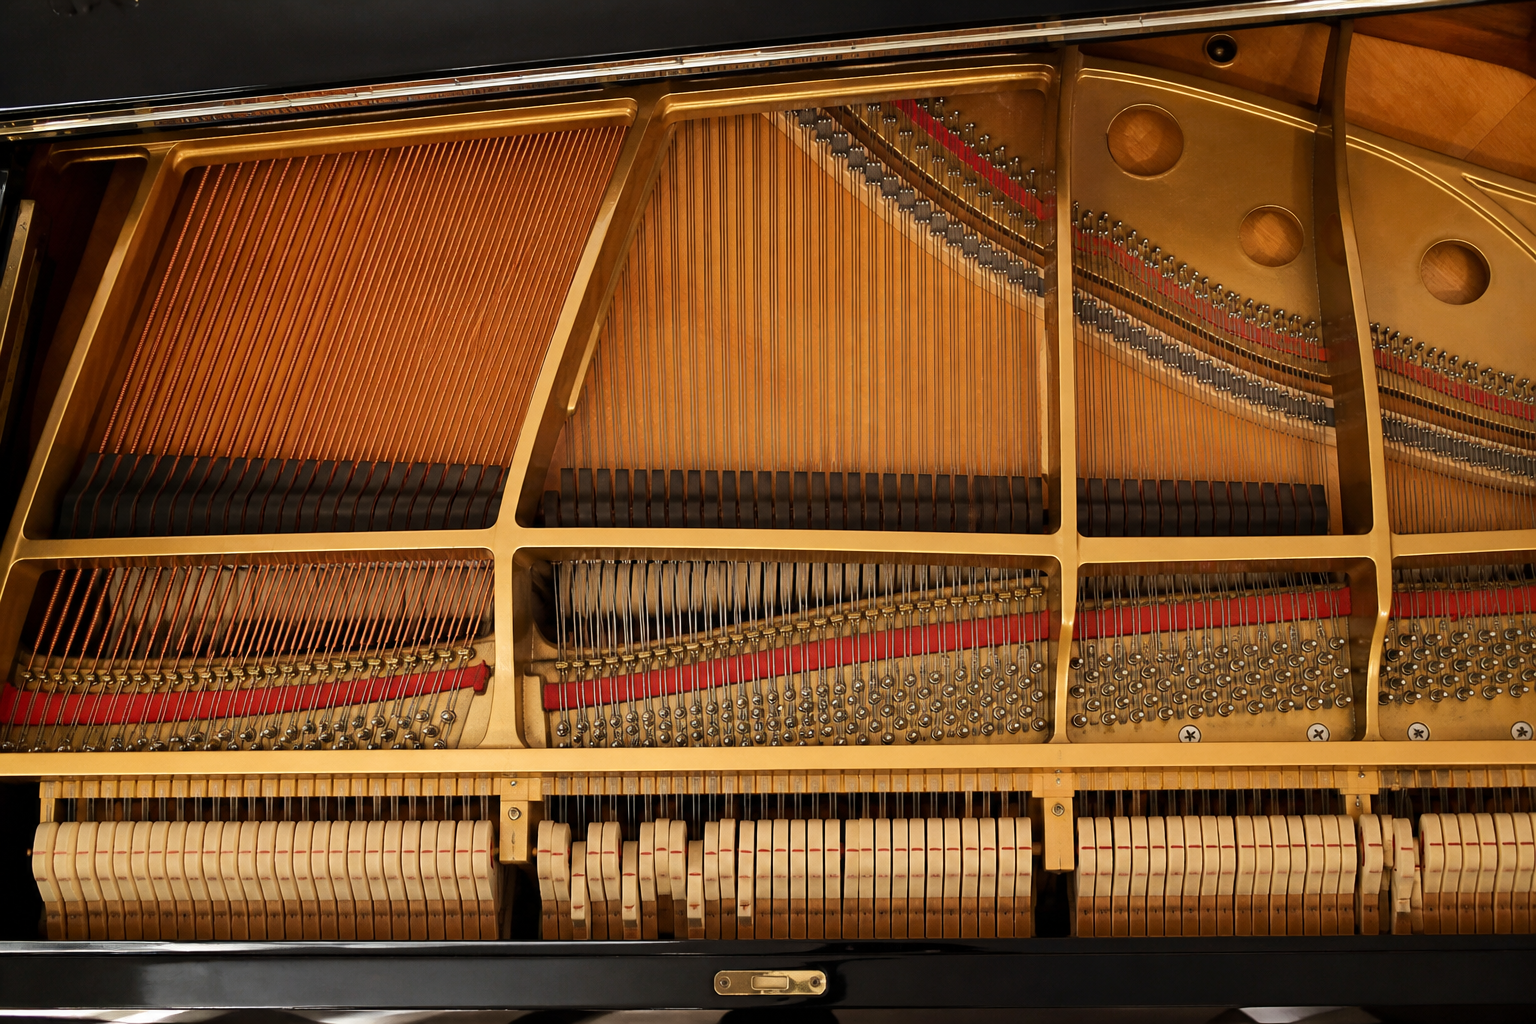
\includegraphics[width=0.58\linewidth]{images/book4/ai/b4-06-grand-piano-strings.png}

{\small داخل بيانو ذي جناح: نحو مئتي وتر فولاذي متدرجة الطول والسماكة، كلٌّ منها موزون بتوتره على نمط أساسي $c/2L$؛ وأوتار الغليظ ملفوفة بالنحاس زيادةً في الكتلة.}
\end{omfigure}

\section{مسألة: البيانو، من المطرقة إلى لوح الرنين}

\begin{problem}[{مسألة نهاية الأسبوع --- وتر بيانو مفكَّك: توتره
وصلابته، وضربة المطرقة والتوافقيات التي تصنعها، والفرس الذي
يسرّب طاقته إلى لوح الرنين، وقضيب سكة يحمل المعادلة نفسها}]
\label{pb:b2:waves-on-strings:1}

\medskip
\noindent\textbf{الجزء I --- الوتر.}
وتر لا$_4$ في بيانو (\qty{440}{Hz}): فولاذ، و $E = \qty{200}{GPa}$، و $\rho =
\qty{7800}{kg/m^3}$، وقطره $d = \qty{1.0}{mm}$، وطوله الناطق $L =
\qty{38}{cm}$. ولكل نغمة فوق الغليظ ثلاثة أوتار كهذه؛ وفي البيانو
$230$ وترًا.
\begin{enumerate}
  \item الكثافة الطولية للكتلة، وسرعة الموجة، وتوتر الوتر.
  \item إجهاد الشدّ في السلك؛ وينكسر السلك عند \qty{2.0}{GPa}: فما
        هامش الأمان، ولماذا تكون لفّة الموازن الأخيرة هي
        الخطرة؟
  \item قدّر التوتر الكلي على الإطار، بأخذ كل الأوتار عند
        التوتر نفسه.
  \item والوتر الأخفض (لا$_0$، \qty{27.5}{Hz}) طوله \qty{1.9}{m}؛ فلو
        كان سلكًا فولاذيًّا صرفًا عند التوتر نفسه، فأي $\mu$ وأي
        قطر يلزمانه؟ وهو في الواقع لبّ فولاذي ملفوف
        بالنحاس: فسّر ذلك.
  \item أنماط وتر لا$_4$: أوجد تواترات التوافقيات الثمانية
        الأولى؛ وأيها يقع على بعد متآلف من النمط الأساسي
        (الديوان، والخماسية، والرباعية، والثالثة الكبيرة) وأيها لا
        يقع؟
  \item يهتزّ الوتر في نمطه الأساسي بسعة
        \qty{0.50}{mm} عند البطن: أوجد الطاقة المخزَّنة (وطاقة
        النمط هي $\tfrac14\mu L\omega^2A^2$).
  \item اكتب النمط الأساسي مجموعَ موجتين منتقلتين؛ وأعطِ
        سعتهما والاستطاعة الوسطى التي تحملها كل منهما.
\end{enumerate}

\medskip
\noindent\textbf{الجزء II --- المطرقة.}
تضرب المطرقة الوتر عند $x_0 = L/8$، فتمنحه، عند $t = 0$،
سرعة $v_0$ على قطعة قصيرة عرضها $w$ حول $x_0$ دون أي
انتقال.
\begin{enumerate}[resume]
  \item اكتب الحلّ العام $y = \sum_nB_n\sin(n\pi x/L)\sin(\omega_nt)$
        وبيّن، باستعمال تعامد الجيوب، أن $B_n =
        \dfrac{2}{L\omega_n}\int_0^L\dot y(x, 0)\sin\dfrac{n\pi x}L\,\dd x$.
  \item ومن أجل ضربة ضيّقة ($w \ll L/n$)، بيّن أن $B_n \approx \dfrac{2v_0w}
        {L\omega_n}\sin\dfrac{n\pi x_0}{L}$.
  \item وأي التوافقيات غائبة من أجل $x_0 = L/8$؟ ولماذا يضرب
        صانعو البيانو قرب $L/7$ إلى $L/8$ (انظر السؤال 5)؟
  \item صف الحركة في صورة الأمواج المنتقلة: ما الذي يغادر
        نقطة الضرب، وماذا يحدث عند الطرفين، وبعد أي زمن
        تتكرر الحالة الابتدائية.
  \item والوتر الحقيقي صلب قليلًا: فأنماطه $f_n = nf_1
        \sqrt{1 + Bn^2}$ حيث $B = \pi^3Ed^4/(64TL^2)$ (مسلَّم بها). احسب
        $B$ وحدّة التوافقي الثامن، بالنسبة المئوية
        وبالسنت (والسنت نسبة تواتر مقدارها $2^{1/1200}$).
  \item ولماذا «يمطّ» موازنو البيانو الديوانات (فيوزنون النغمات
        العالية أحدّ قليلًا)؟
\end{enumerate}

\medskip
\noindent\textbf{الجزء III --- الفرس ولوح الرنين.}
يعبر الوتر فرسًا ملصوقًا بلوح الرنين؛ ويسلك لوح الرنين،
عند الفرس، سلوك وتر ممانعته $Z_b = \qty{2000}{kg/s}$.
\begin{enumerate}[resume]
  \item ممانعة الوتر $Z_s$؛ ومعامل الانعكاس في السعة
        عند الفرس.
  \item النسبة المنقولة من طاقة الموجة إلى لوح الرنين عند
        كل انعكاس.
  \item عدد الانعكاسات في الثانية عند الفرس؛ واستنتج ثابت
        الزمن لتخامد الطاقة والزمن اللازم كي يهبط الصوت
        \qty{60}{dB} (أي بمعامل $10^6$ في الطاقة).
  \item الاستطاعة المتسرّبة إلى لوح الرنين بُعيد ضربة
        السؤال 6؛ وقارنها باستطاعة حديث هادئ، وهي
        نحو \qty{1e-5}{W} من الصوت.
  \item ولماذا يكاد الوتر وحده لا يُسمع، وما الذي يفعله لوح
        الرنين حيال ذلك؟ (فكّر في ممانعة الهواء،
        $\rho c \approx \qty{400}{kg.m^{-2}.s^{-1}}$، منظورةً عبر سطح
        صغير مقابل سطح كبير.)
  \item وبرفع المخمّد، يبدأ وتر لا$_3$ (\qty{220}{Hz}) بالصوت
        حين يُعزف لا$_4$: فلماذا؟
  \item ويريد صانع بيانو دوامًا أطول للصوت: أينبغي رفع $Z_b$ أم
        خفضها، وما الذي يُفقَد؟
\end{enumerate}

\medskip
\noindent\textbf{الجزء IV --- قضيب السكة.}
قضيب سكة فولاذي ($E = \qty{200}{GPa}$، و $\rho = \qty{7800}{kg/m^3}$، ومقطعه
\qty{70}{cm^2}).
\begin{enumerate}[resume]
  \item سرعة أمواج الانضغاط؛ والزمن الذي يستغرقه صوت قطار في
        قطع \qty{5}{km} على امتداد القضيب وعبر الهواء.
  \item وتُرسل ضربة مطرقة نبضة انضغاط في قطعة قضيب طولها
        \qty{25}{m} ذات طرف حرّ: أوجد زمن الصدى؛ وهل الصدى
        انضغاط أم تخلخل؟
  \item ويبحث مسبار فوق صوتي عند \qty{2}{MHz} عن الشروخ: أوجد طول
        الموجة في الفولاذ؛ ومعامل الانعكاس في السعة عند شرخ
        بين الفولاذ والهواء (وممانعة الهواء $\qty{400}{kg.m^{-2}.s^{-1}}$)؛
        ولماذا يُرى الشرخ الرقيق بهذا الوضوح.
  \item الزلازل: تنتقل أمواج الانضغاط في الصخر بالسرعة
        \qty{6.0}{km/s} وأمواج القصّ بالسرعة \qty{3.5}{km/s}. وتسجّل محطة
        موجة القصّ بعد موجة الانضغاط بمقدار \qty{20}{s}: فما بعد
        المصدر؟
  \item اجمع في جدول واحد سرعات الأمواج الخمس في هذه المسألة
        (الوتر، والقضيب، والانضغاط في الصخر، والقصّ في الصخر،
        والهواء) مع الصلابة والعطالة اللتين تحدّدان كلًّا منها.
\end{enumerate}
\end{problem}
